
\chapter{Simulation study} 

\label{simulation-study}

A sizable Monte-Carlo simulation study has been carried out to test the performance, accuracy and computational efficiency of the three presented estimators (maximum likelihood, Kendall's Tau inversion and Blomqvist's Beta inversion) in terms of copulae parameter estimation and selecting an appropriate copula from data. To measure parameter-estimation-accuracy, the mean-square-error (MSE) for every parameter estimate per estimator is calculated and averaged over a large number of experiments. The performance is determined via relative computation time it takes for my algorithm to converge. I do not use absolute values, because they carry no additional information about computational performance but much rather about the specific hardware I am using.

In terms of selecting one copula for a given set of data, relative computation time for my algorithm to converge to one copula is measured per estimator. The validity of its choice is also denoted.

\section{Procedure}

The design of this simulation study will base on several other studies that measure performance of different parameter estimators for copulae in a Monte-Carlo manner such as \citet{kim2007comparison}, \citet{kojadinovic2010comparison}, \citet{weiss2011copula} or \citet{genest2013copula}.

For every parametric copula presented above the following steps are repeated $k$ times in sequence fr the parameter estimation:

\begin{enumerate}
	\itemsep0em
	\item A sample of size $n$ is simulated from a theoretical copula $C \in (C_\theta)$ with true parameter $\theta$.
	\item Compute the parameter estimates with the maximum-likelihood and each of the moment-based inverses under the premise that the parametric form of the copula is known.
	\item Calculate the average MSE per parameter by $MSE(\hat{\boldsymbol{\theta}}) \equiv k^{-1}   \sum_{i=1}^{k} E\left[ \theta - \hat{\boldsymbol{\theta}}_i \right]^2 $, with $\theta$ being the true parameter and $\hat{\boldsymbol{\theta}}$ being the estimated parameter vector from equation \ref{estimators} for every iteration.
	\item Provide relative computation time per estimator per copula, where median maximum-likelihood time is set to 100 ($\tilde{t}_{ML} = 100$). All benchmarking exercises are done using the \verb*|microbenchmark| package.
\end{enumerate}

For this study I will set $k = 1000$ and $ n = \left\lbrace 30,50,100 \right\rbrace $ similar to other studies provided above. The optimization process for maximum-likelihood uses a bounded, limited-memory BFGS algorithm, which has been proven to be an optimal choice for maximum entropy problems \citep{malouf2002comparison}. I will test the whole process for a range of parameter values. For the elliptical copulae I use $\rho \in \left\lbrace -0.9,-0.8 \dots 0.8,0.9 \right\rbrace $ while for the archimedean copulae I use $\theta \in \left\lbrace 1,1.5 \dots 9.5,10 \right\rbrace $. I will set the degrees of freedom for the $t$-copula fix to $\nu = 4$ as it drastically increases computational speed since the estimation process for the degrees of freedom can be circumvented \citep{lucas2014conditional}. 

The copula selection process will follow a similar fashion as the parameter estimation. The following process is repeated $k$ times:

\begin{enumerate}
	\itemsep0em
	\item A sample of size n is simulated from a known copula $C \in (C_\theta)$ with known parameter $\theta$.
	\item The sample is fitted to every copula available for each estimator and respective AIC values are computed.
	\item Copula with lowest AIC per estimator is chosen. Correct selections over $k$ are returned ($\frac{\# \text{of correct selections}}{k}$).
	\item Relative computation times per copula and estimator are computed. Again done with the \verb*|microbenchmark| package.
\end{enumerate}

During the copula selection procedure, I use $k = 100$ and  $ n = \left\lbrace 30,100 \right\rbrace $. As with the parameter estimation, the range of parameters per copula and estimator will remain the same.

The simulation is performed on version \verb*|4.0.3| of \verb*|R|. The copula observations are simulated using the \verb*|BiCopSim| function from the \verb*|VineCopula| package.

\section{Results}

The results of the parameter estimation study are shown in Figures \ref{gauss_t_sim}, \ref{clayton-gumbel-sim} and \ref{frank-sim}. Relative computation time can be found in table \ref{rel-comp-time-est}. The figures show the average mean-square-error for every estimator and parameter for $1000$ repetitions per parameter step. The sample size $n = 50$ is omitted in the figures as the result is congruent with the evidence showing that accuracy increases with sample size for all estimators.

\subsection{Estimator choice for parameter estimation}

Interestingly, the results show a relatively uniform behavior for the inversion of Kendall's Tau and maximum likelihood estimators. Regardless of the magnitude of dependence, both estimators show very small MSEs across all parameters with Tau's inversion being slightly inferior in high dependence scenarios for archimedean copula where $\theta > 6$. 

The relative computation times from Table \ref{rel-comp-time-est} reveal that, although being approximately equally accurate, Kendall's Tau inversion can be more than ten times faster than maximum likelihood. This outcome occurs when the density functions of the respective copulae are computationally challenging as for example with the $t$-copula. Vice versa, in scenarios where there is no closed form relationship function between the copula and its dependence measure, computation time is almost equal, i.e Tau inversion for the Frank copula still needs $92.3\%$ of the time it takes ML to converge.

Blomqvist's Beta inversion is not recommended to use for parameter estimation under any circumstance. It may be faster to compute in some situations, however, the large margin of error can make predictions error-prone and unpredictable. This is especially evident in extreme value copulae such as the Gumbel copula, with MSE values exceeding ten.

\begin{figure}[!ht]
	\subfloat{%
		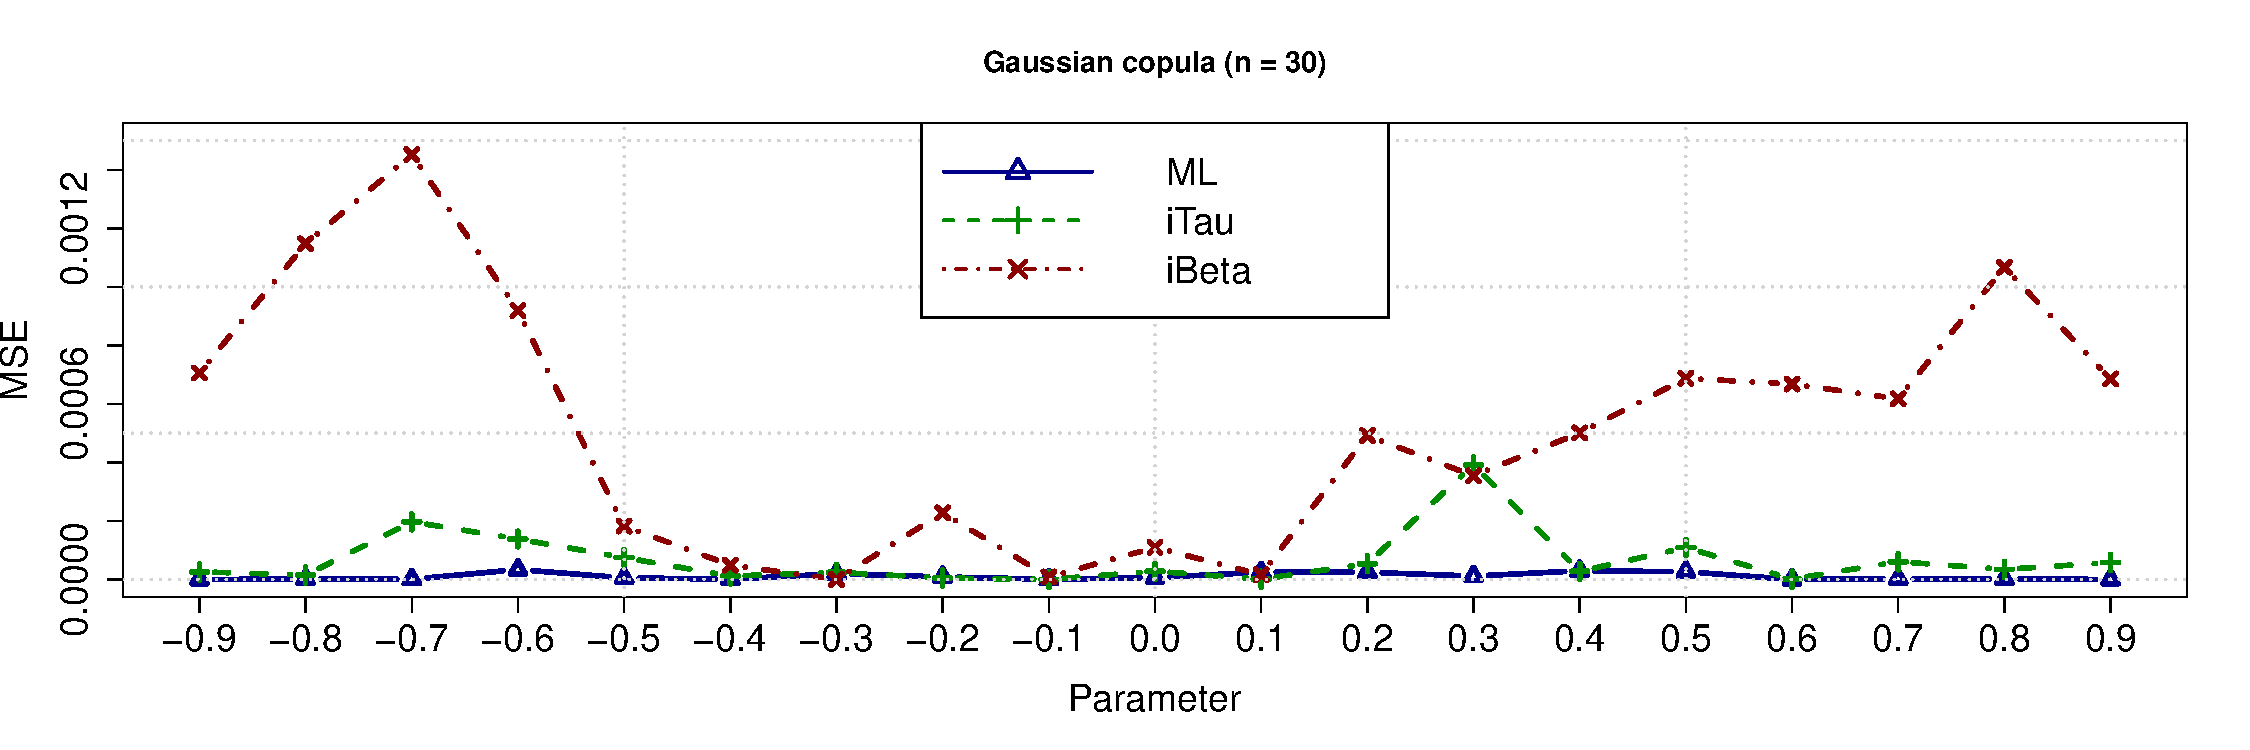
\includegraphics[trim= 0cm 1.6cm 1cm 0cm, width = .98\textwidth]{Figures/mc-plots/gaussian30.pdf}
	}
	\hfill
	\subfloat{%
		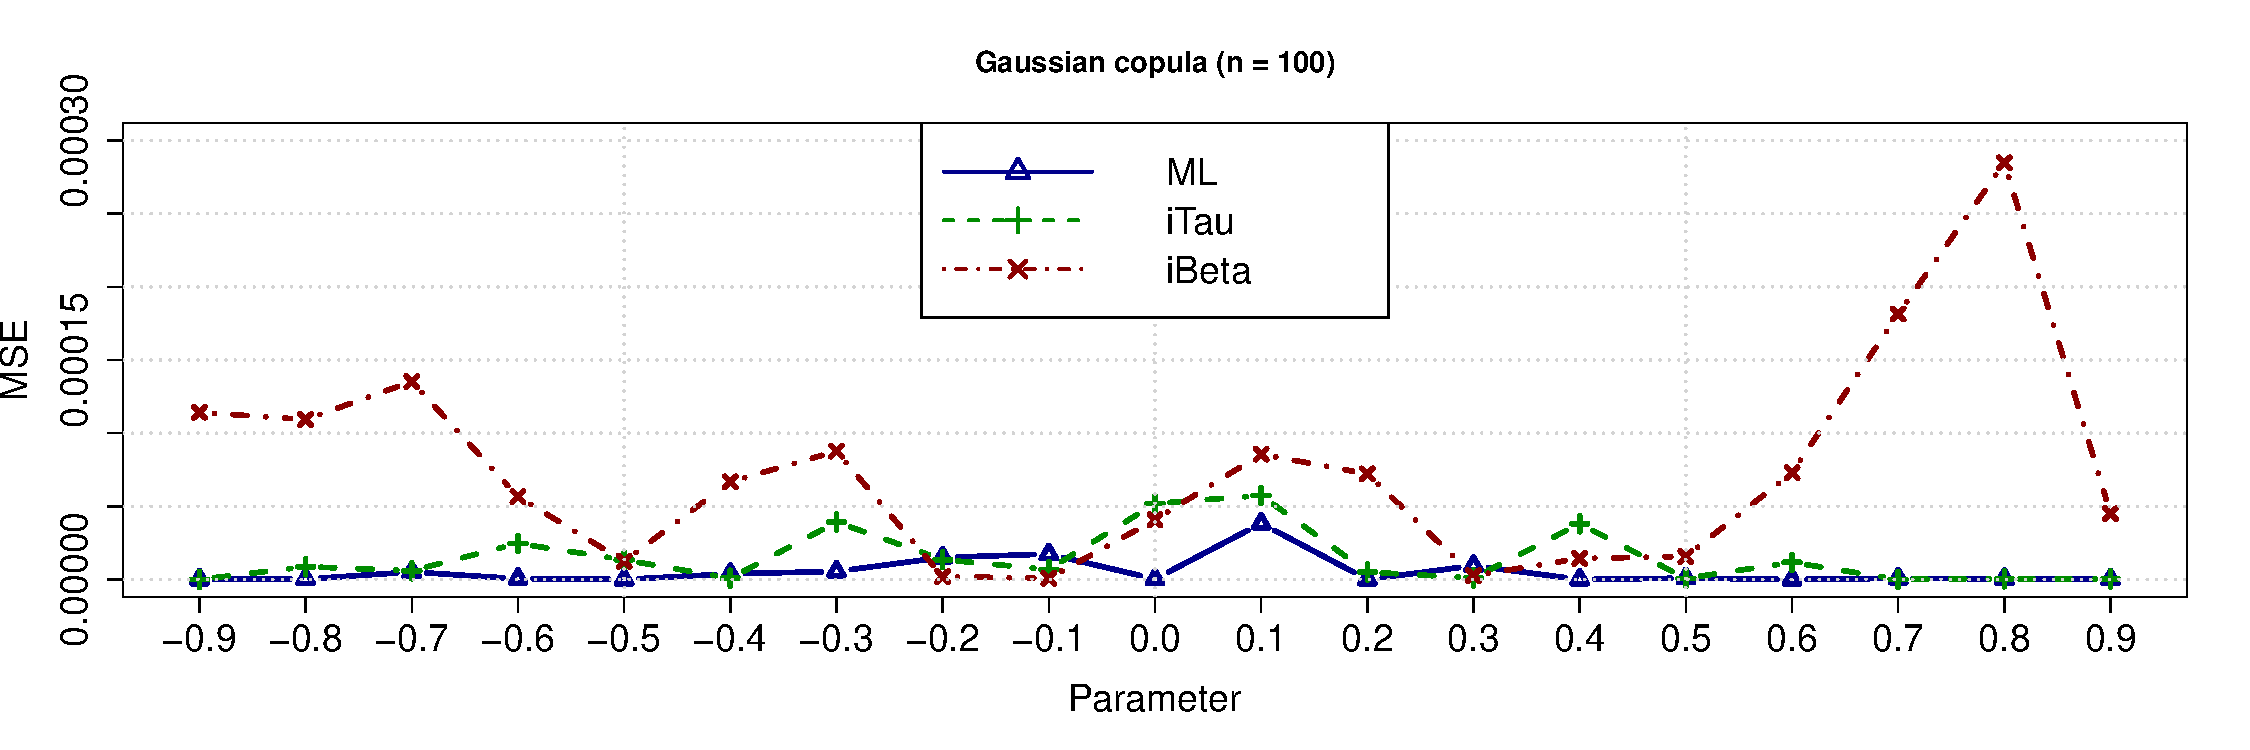
\includegraphics[trim= 0cm 1.6cm 1cm 0cm,width = .98\textwidth]{Figures/mc-plots/gaussian100.pdf}
	}
	\hfill
	\subfloat{%
		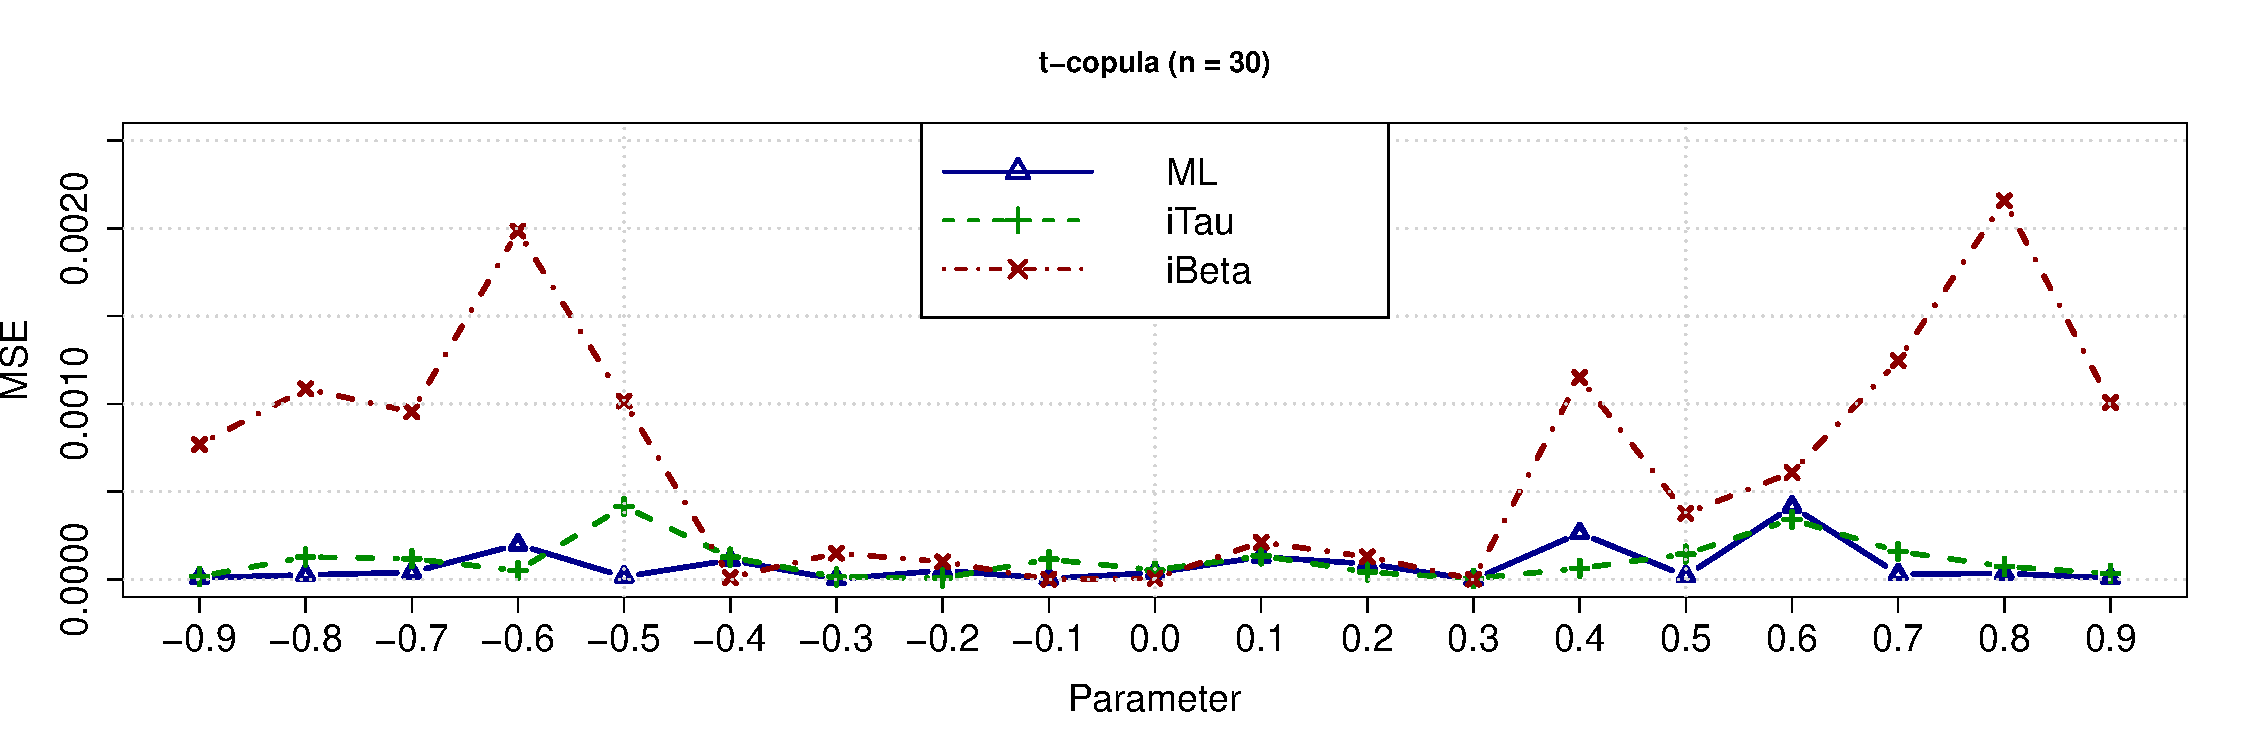
\includegraphics[trim= 0cm 1.6cm 1cm 0cm, width = .98\textwidth]{Figures/mc-plots/t30.pdf}
	}
	\hfill
	\subfloat{%
		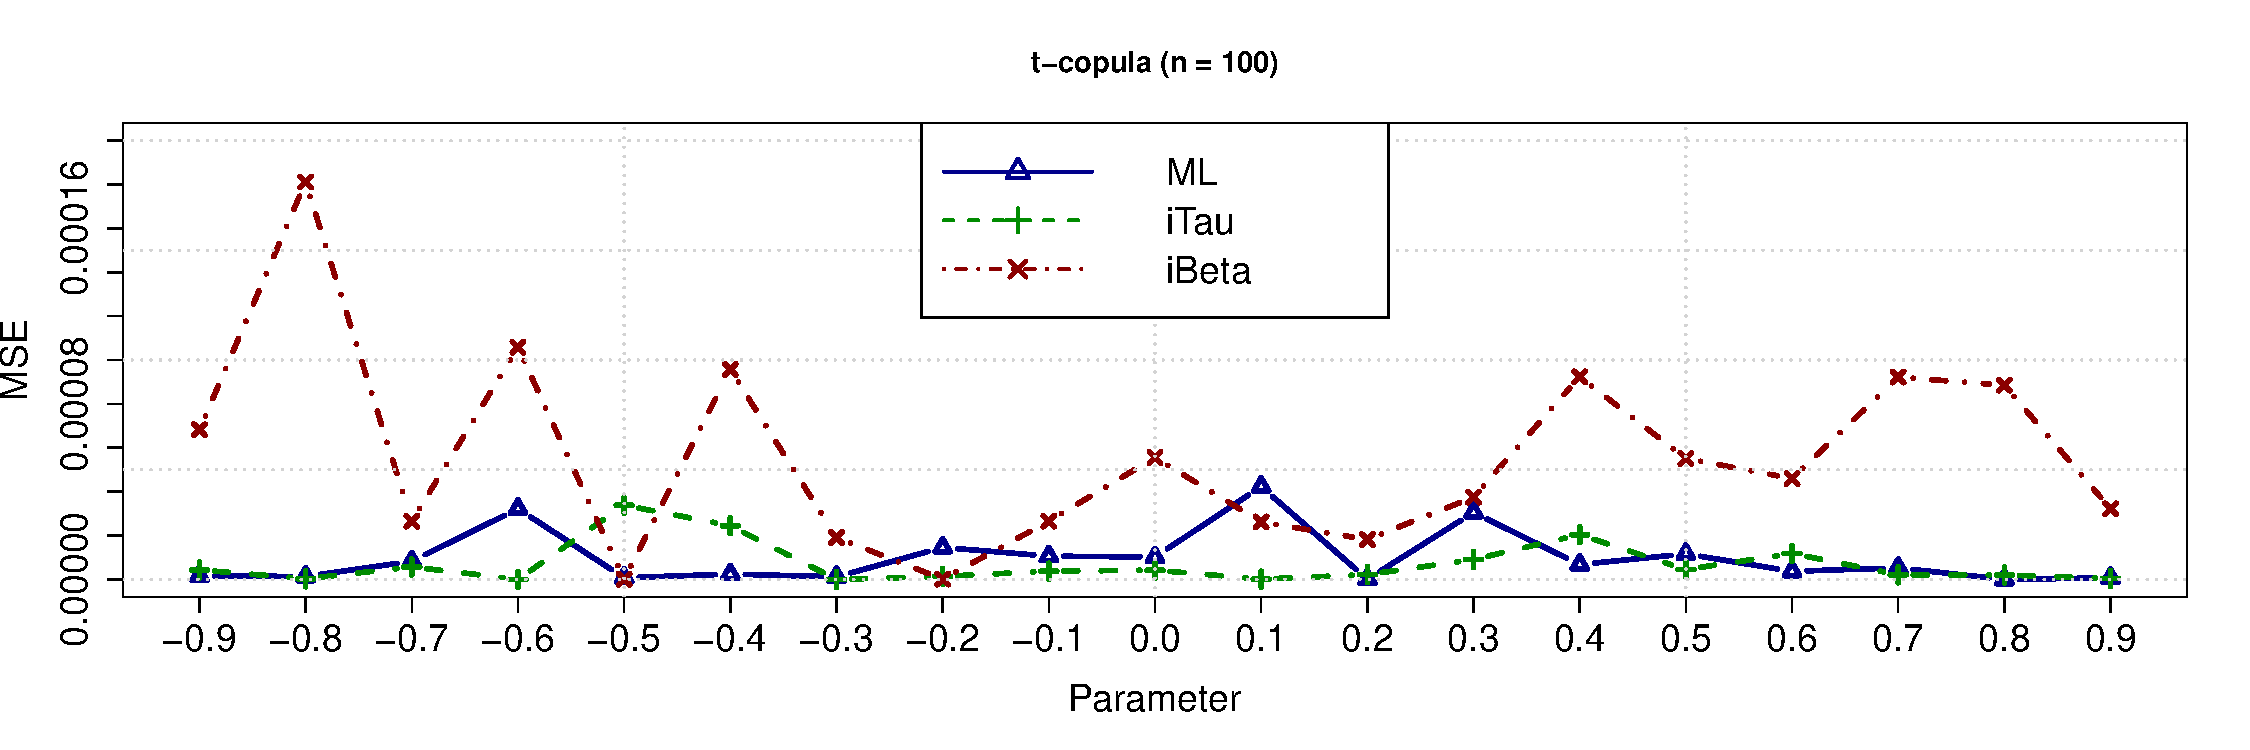
\includegraphics[trim= 0cm 1cm 1cm 0cm, width = .98\textwidth]{Figures/mc-plots/t100.pdf}
	}
	\caption[\textsc{Simulation results for Gaussian and $t$-copula}]{Mean square error for the maximum-likelihood (ML) and both inversion methods for different copulae and parameters. Sample size alternates between  $ n = \left\lbrace 30,100 \right\rbrace $ and $k = 1000$. It is assumed here that the simulated data comes from a true known copula.}
	\label{gauss_t_sim}
\end{figure}

\begin{figure}[!ht]
	\subfloat{%
		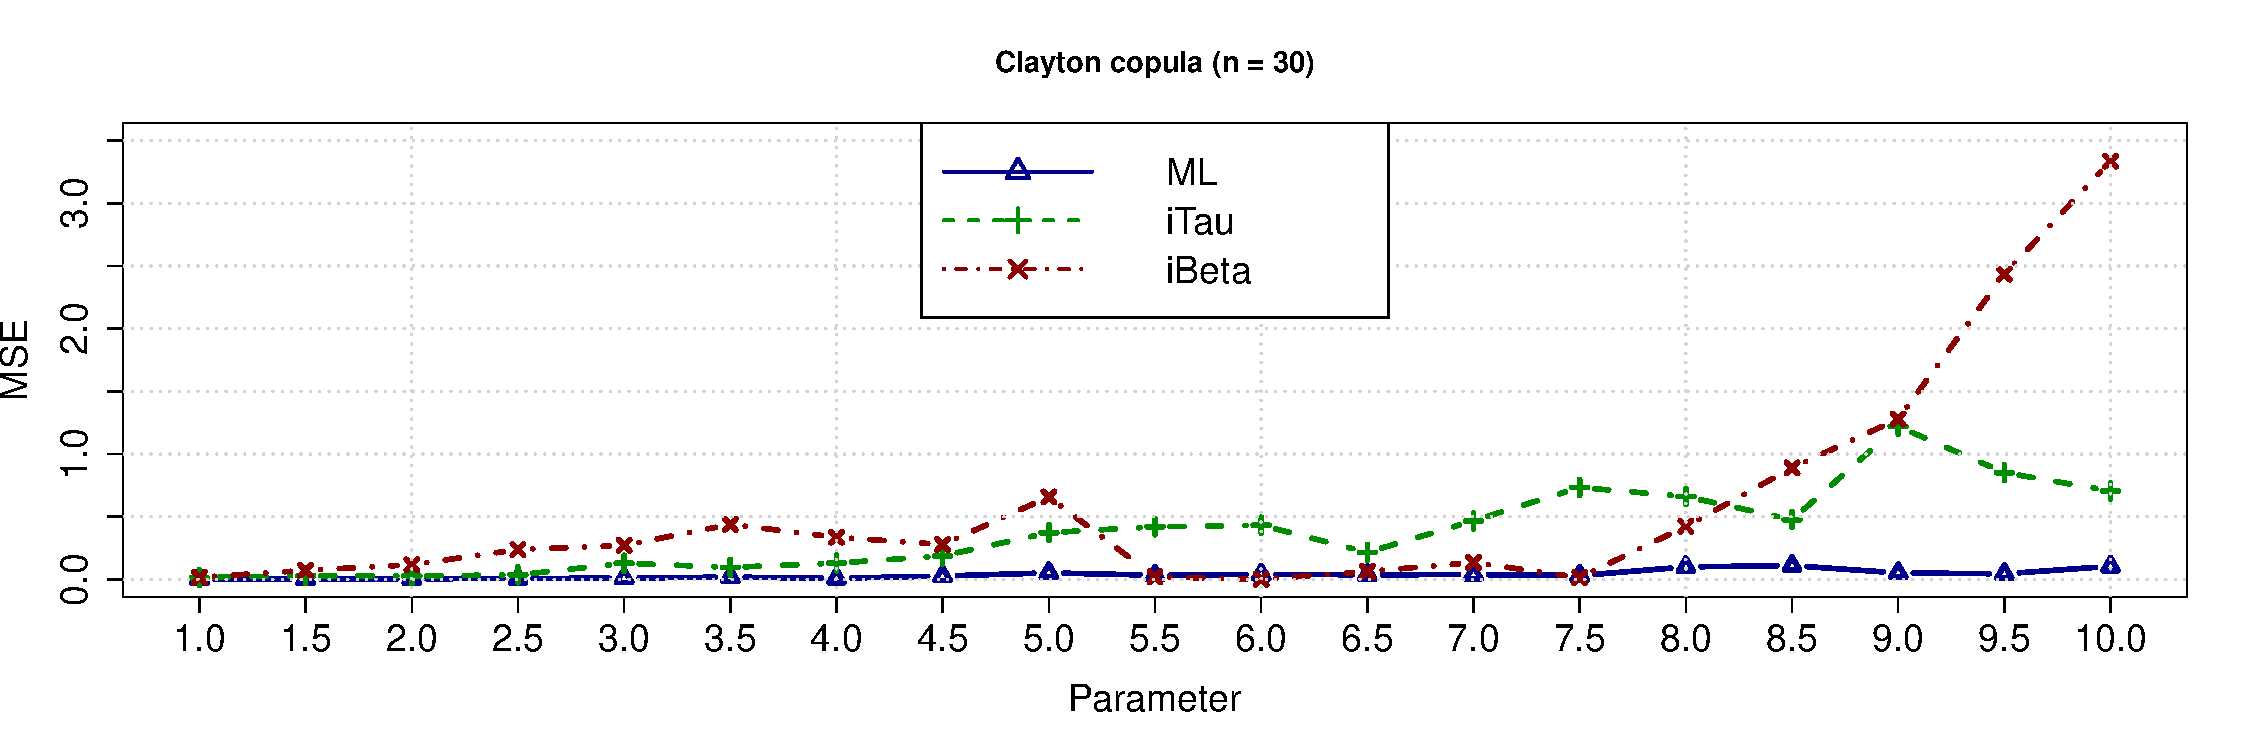
\includegraphics[trim= 0cm 1.6cm 1cm 0cm, width = .98\textwidth]{Figures/mc-plots/clayton30.pdf}
	}
	\hfill
	\subfloat{%
		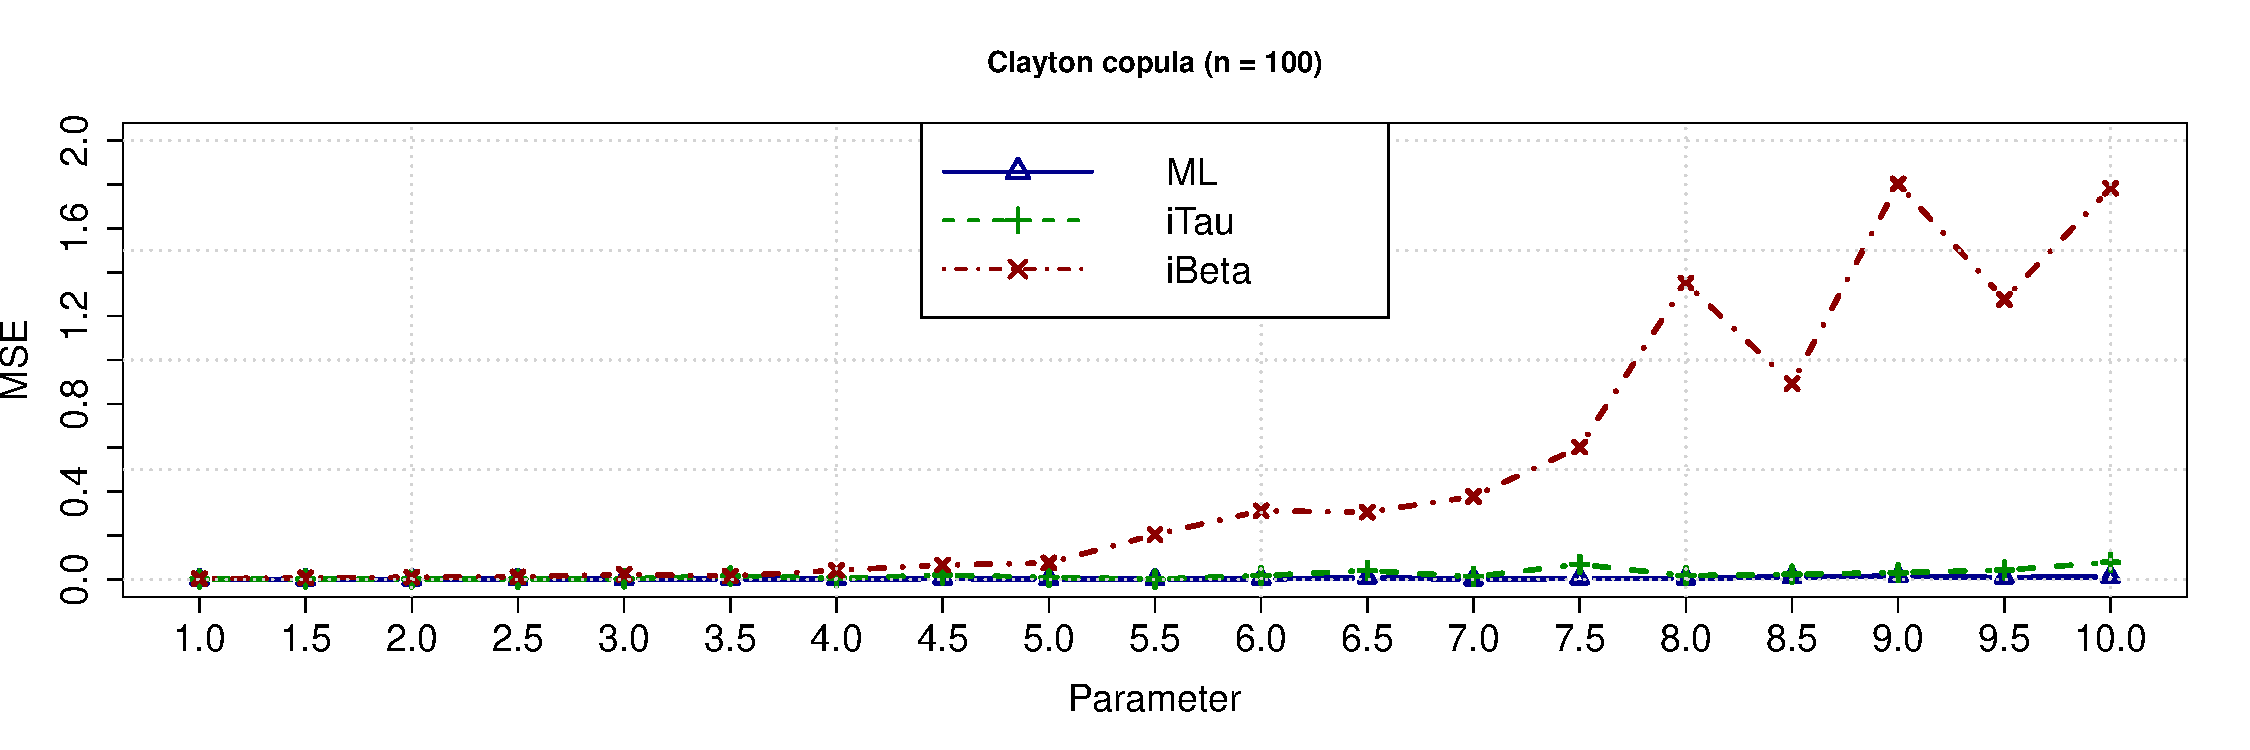
\includegraphics[trim= 0cm 1.6cm 1cm 0cm,width = .98\textwidth]{Figures/mc-plots/clayton100.pdf}
	}
	\hfill
	\subfloat{%
		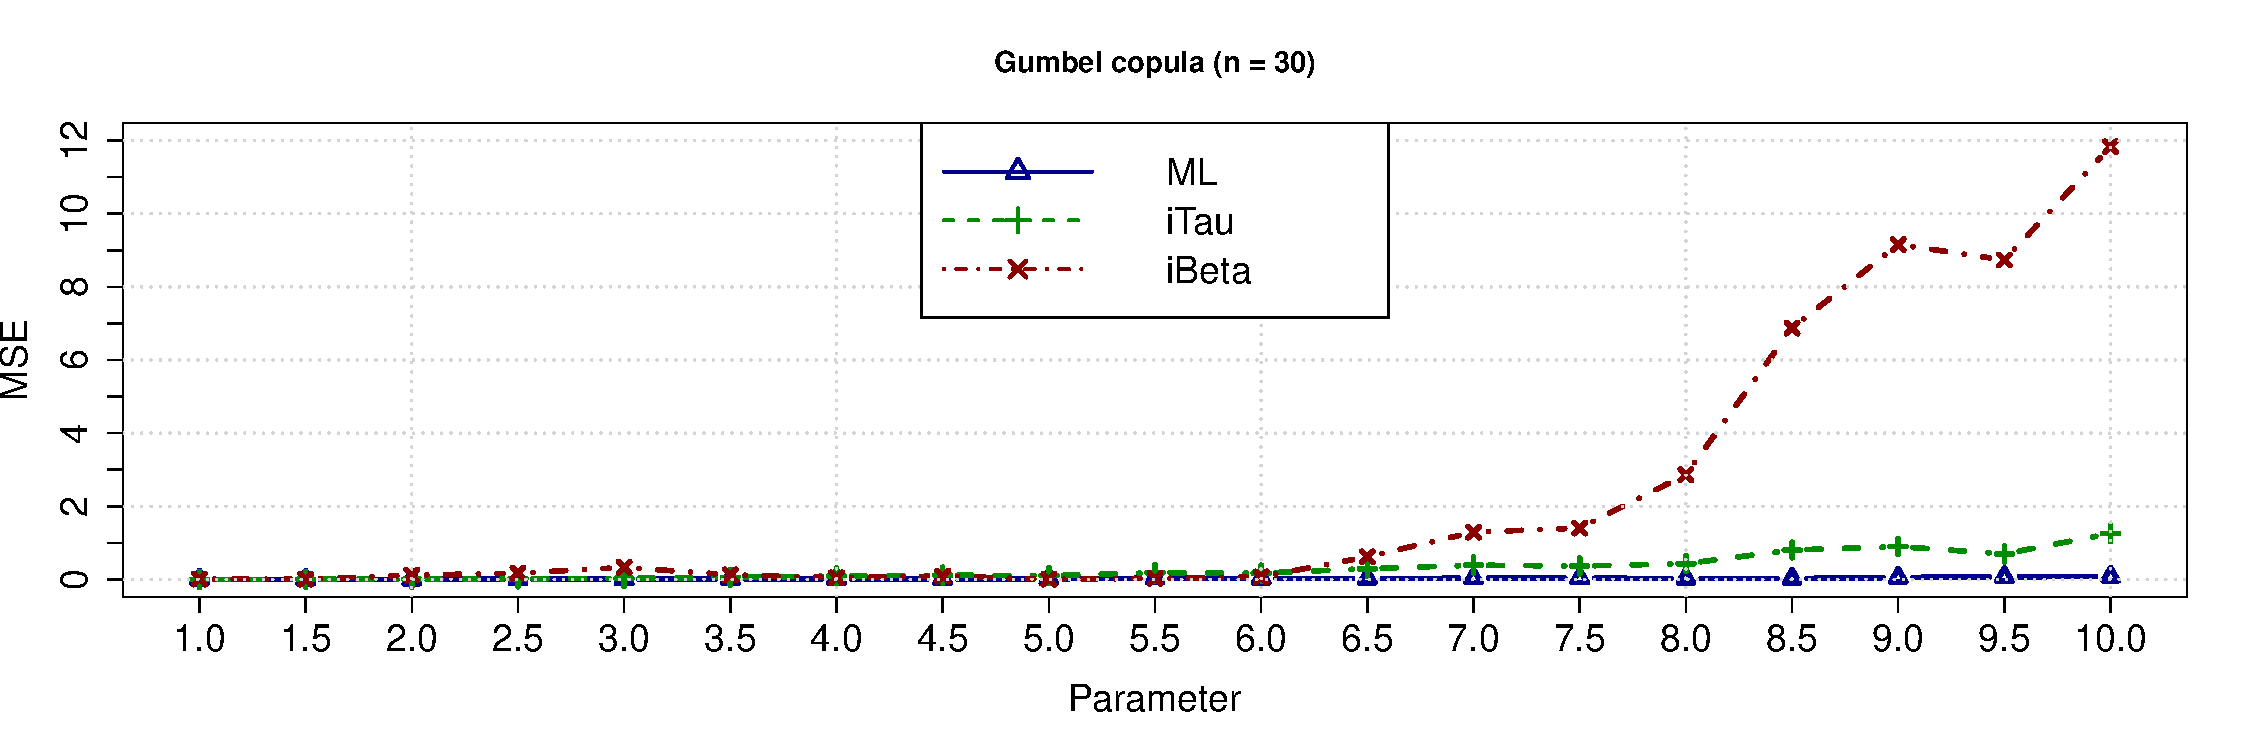
\includegraphics[trim= 0cm 1.6cm 1cm 0cm, width = .98\textwidth]{Figures/mc-plots/gumbel30.pdf}
	}
	\hfill
	\subfloat{%
		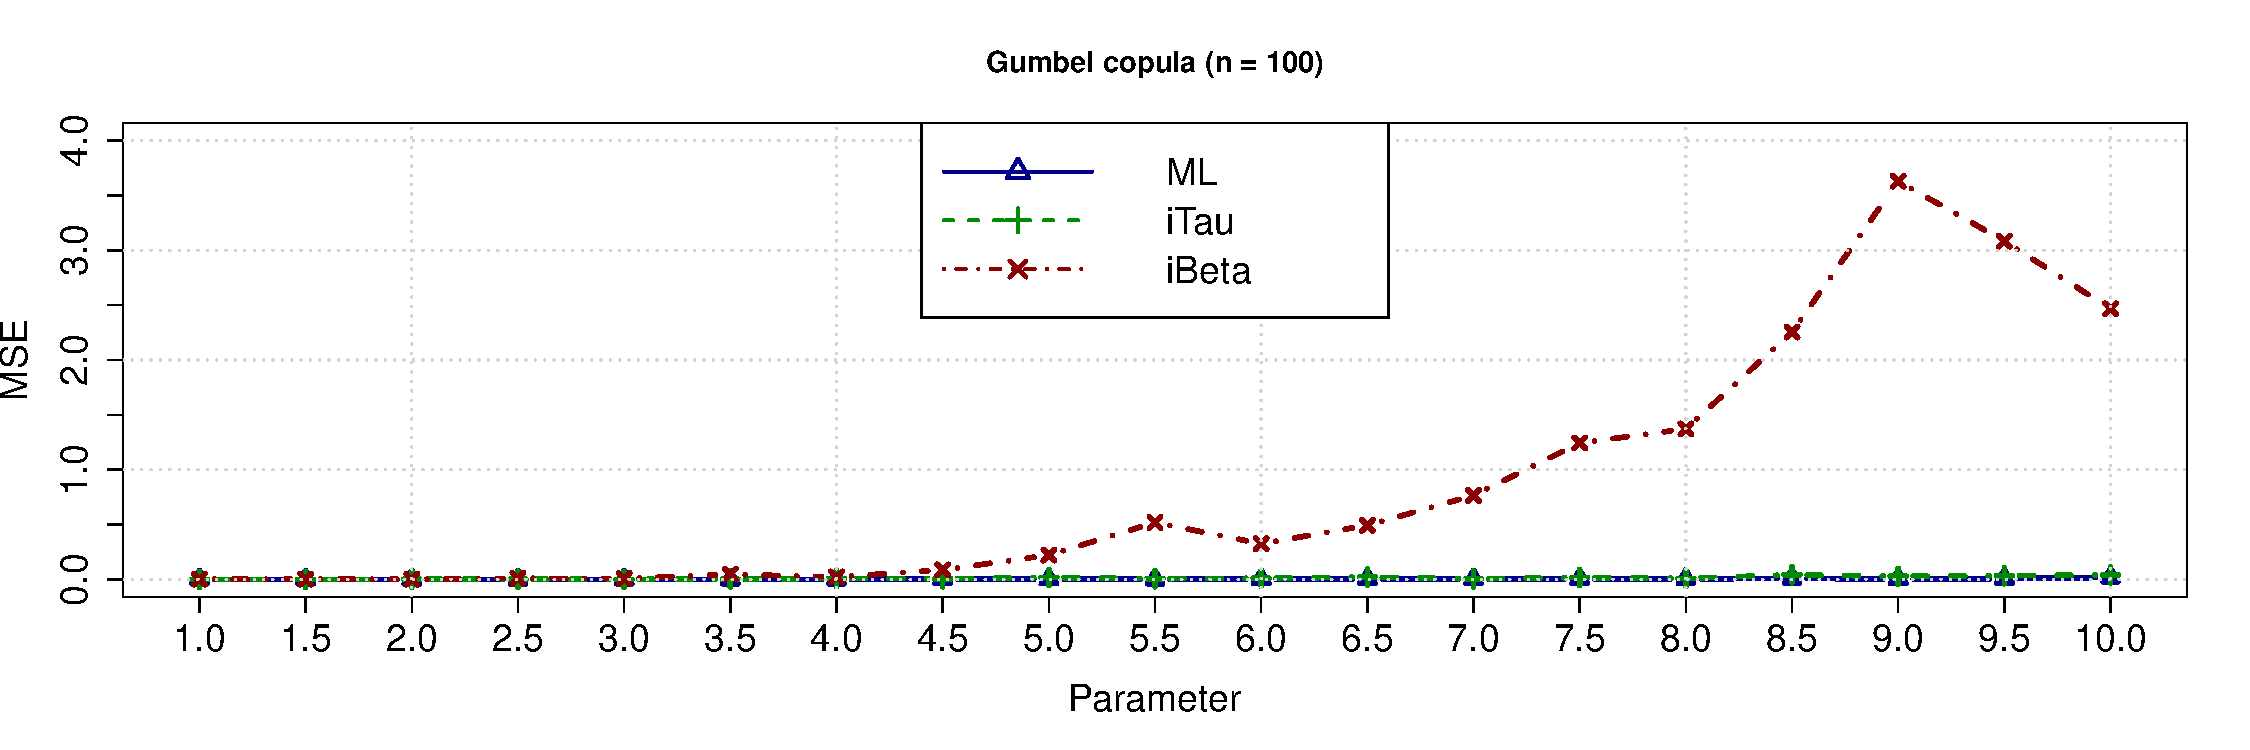
\includegraphics[trim= 0cm 1cm 1cm 0cm, width = .98\textwidth]{Figures/mc-plots/gumbel100.pdf}
	}
	\caption[\textsc{Simulation results for Clayton and Gumbel copula}]{Continuation of Figure \ref{gauss_t_sim} for the Clayton and Gumbel copula.}
	\label{clayton-gumbel-sim}
\end{figure}

\begin{figure}[!ht]
	\subfloat{%
		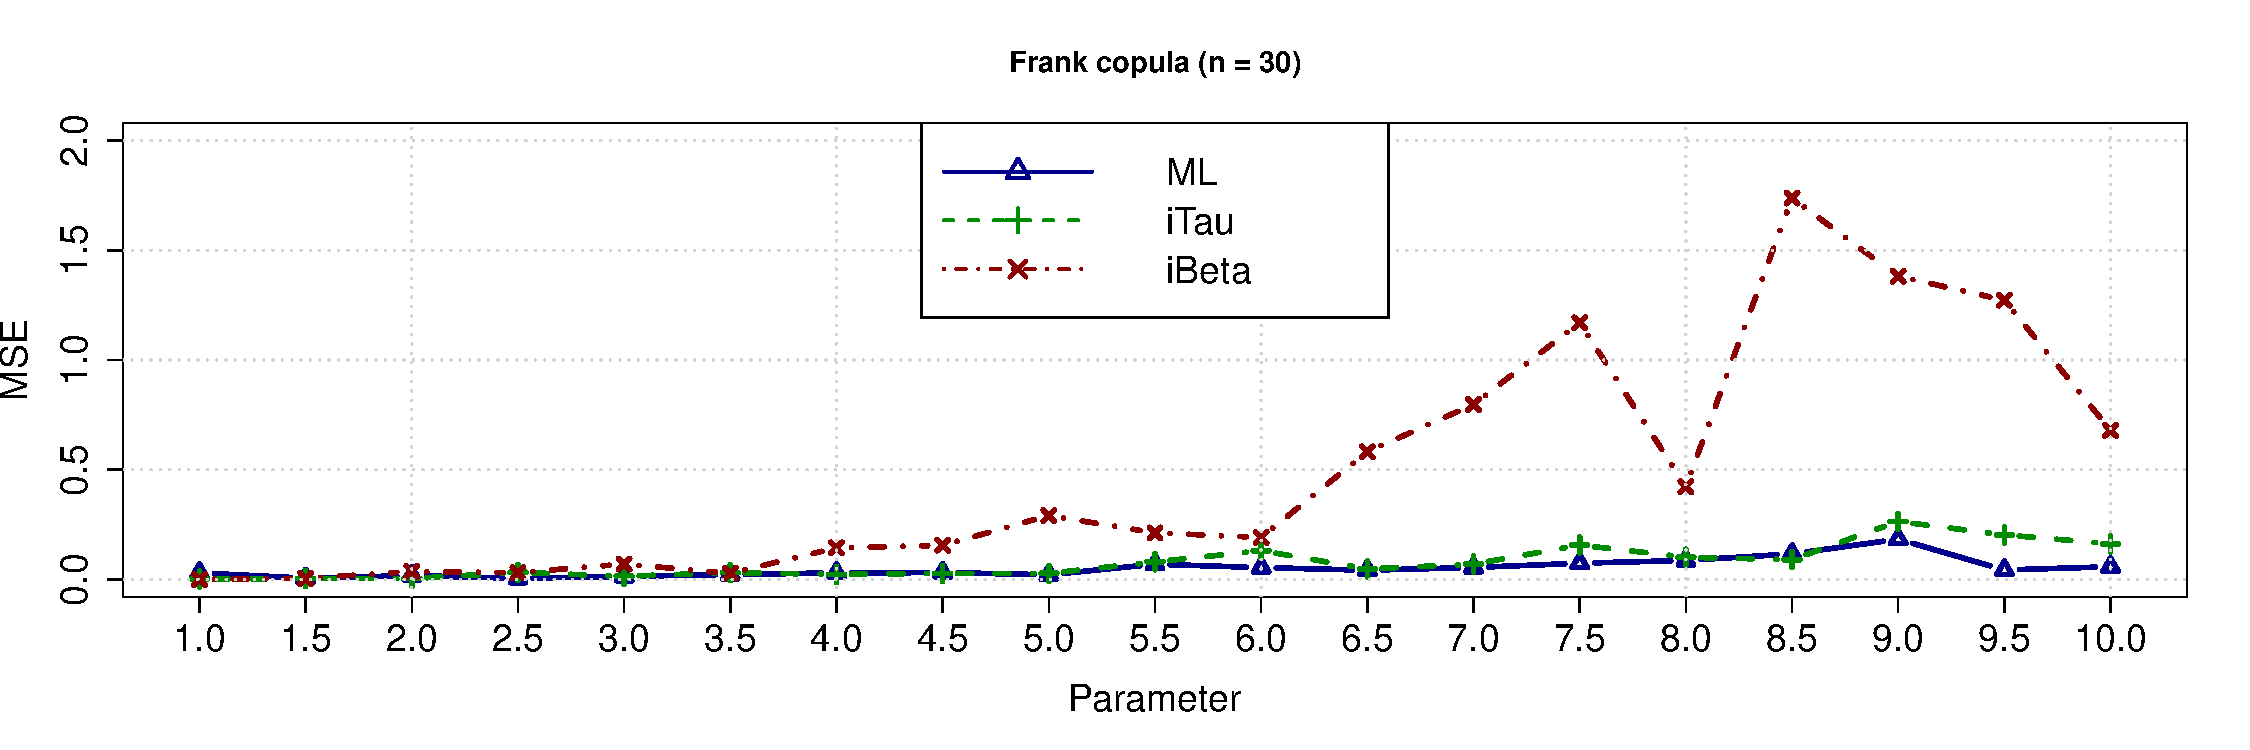
\includegraphics[trim= 0cm 1.6cm 1cm 0cm, width = .98\textwidth]{Figures/mc-plots/frank30.pdf}
	}
	\hfill
	\subfloat{%
		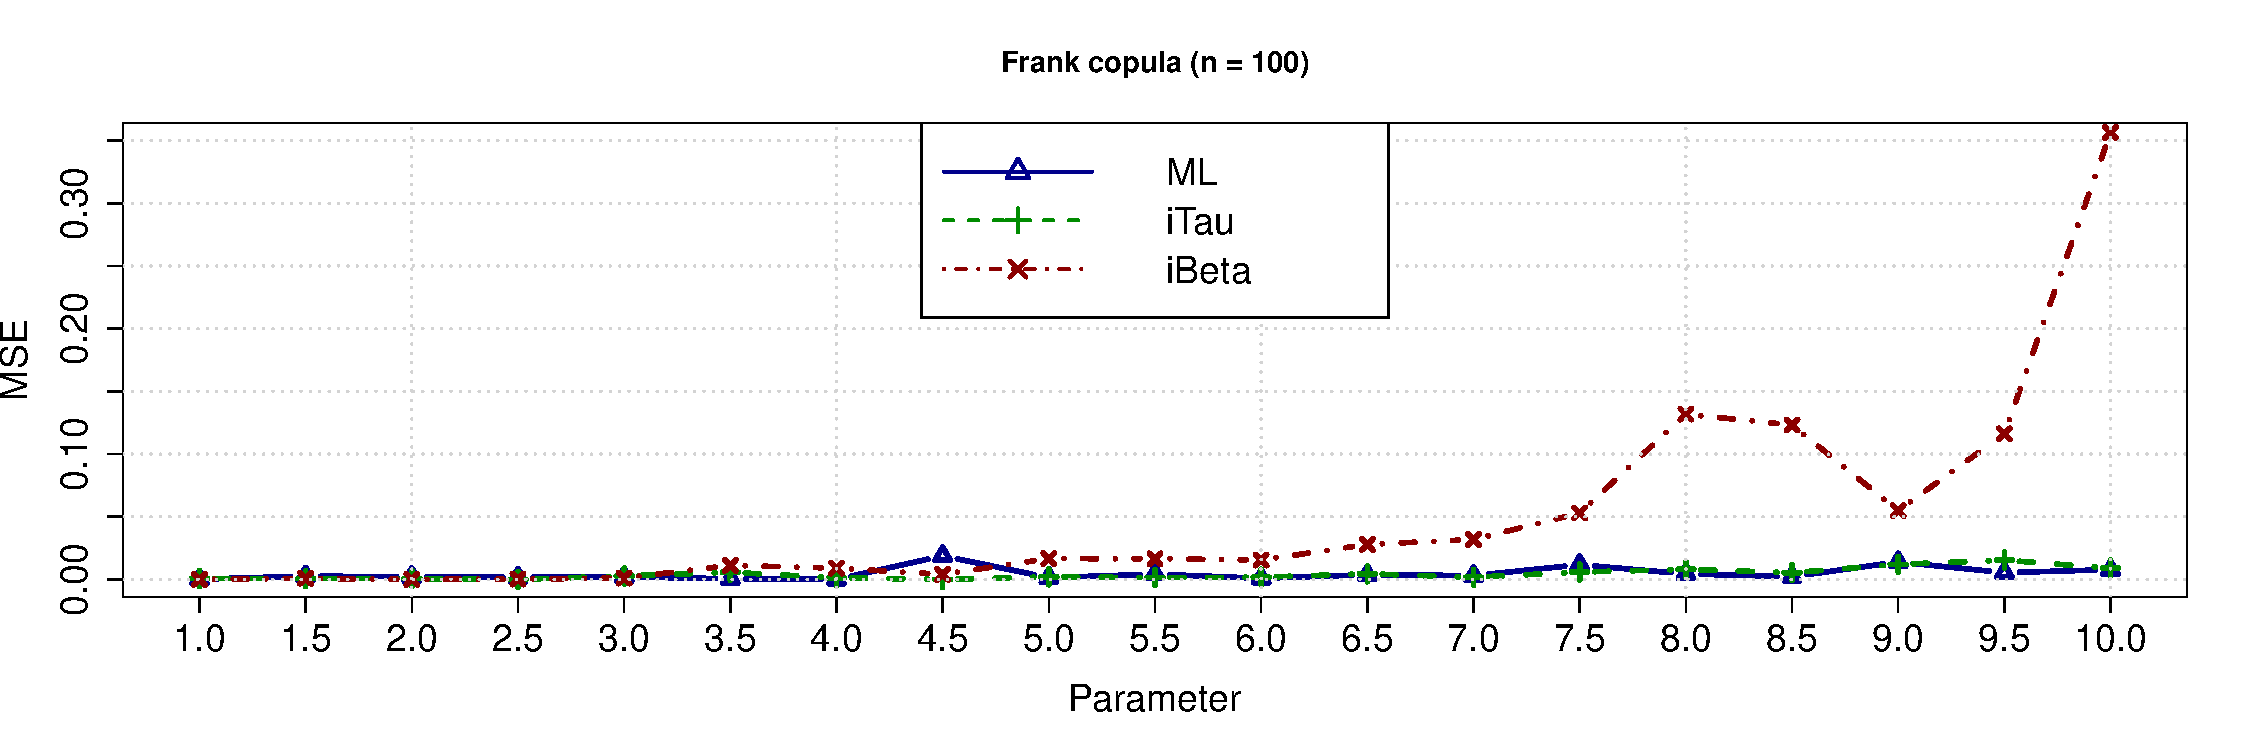
\includegraphics[trim= 0cm 1cm 1cm 0cm,width = .98\textwidth]{Figures/mc-plots/frank100.pdf}
	}
	\caption[\textsc{Simulation results for Frank copula}]{Continuation of \ref{gauss_t_sim} and \ref{clayton-gumbel-sim} for the Frank copula.}
	\label{frank-sim}
\end{figure}

\begin{table}[h!]
	\centering
{\renewcommand{\arraystretch}{1.3}
	\begin{tabular}{ll|ccc}
		Copula family             & Estimator & $\min_t$   & $\tilde{t}$ & $\max_t$   \\ \hline \hline
		\multirow{3}{*}{Gaussian} & ML        & 0.996 & 1.000      & 1.051 \\
		& iTau      & 0.146 & 0.147  & 0.148 \\
		& iBeta     & 0.182 & 0.183  & 0.185 \\ \hline
		\multirow{3}{*}{t}        & ML        & 0.989 & 1.000      & 1.045 \\
		& iTau      & 0.032 & 0.032  & 0.033 \\
		& iBeta     & 0.035 & 0.035  & 0.036 \\ \hline
		\multirow{3}{*}{Clayton}  & ML        & 0.992 & 1.000      & 1.006 \\
		& iTau      & 0.152 & 0.155  & 0.157 \\
		& iBeta     & 0.247 & 0.248  & 0.251 \\ \hline
		\multirow{3}{*}{Gumbel}   & ML        & 0.999 & 1.000      & 1.002 \\
		& iTau      & 0.113 & 0.114  & 0.114 \\
		& iBeta     & 0.139 & 0.140  & 0.141 \\ \hline
		\multirow{3}{*}{Frank}    & ML        & 0.997 & 1.000      & 1.006 \\
		& iTau      & 0.922 & 0.923  & 0.925 \\
		& iBeta     & 0.909 & 0.910  & 0.917
	\end{tabular}
}
\caption[Relative computation time per estimator and copula for parameter estimation.]{Relative computation time per copula and estimator. For the benchmark I calculated the average time it takes the algorithm to converge to a parameter. I use $n = 100$ and $k = 5000$.}
\label{rel-comp-time-est}
\end{table}

\subsection{Estimator choice for copula selection}

Figures \ref{copSelect-gauss-t} and \ref{copSelect-gumbel-frank} depict the accuracy of each estimator copula and parameter for the selection process based the AIC for $ n = \left\lbrace 30,100 \right\rbrace $ and $k = 100$. Surprisingly, all estimators seem to perform equally in terms of selecting a copula, given a set of data. The difference in computation time between the estimators from Table \ref{comp-time-seletion}, however, is noteworthy. Even for the smallest sample size $n = 30$, there is no notable difference in accuracy across all copulae and parameters, yet the inversion methods are at least 16 times faster than maximum-likelihood. This is most likely due to skipped optimization process for the inversion methods, as no first- or second-order derivatives need to be calculated.



\begin{figure}[t]
	\subfloat{%
		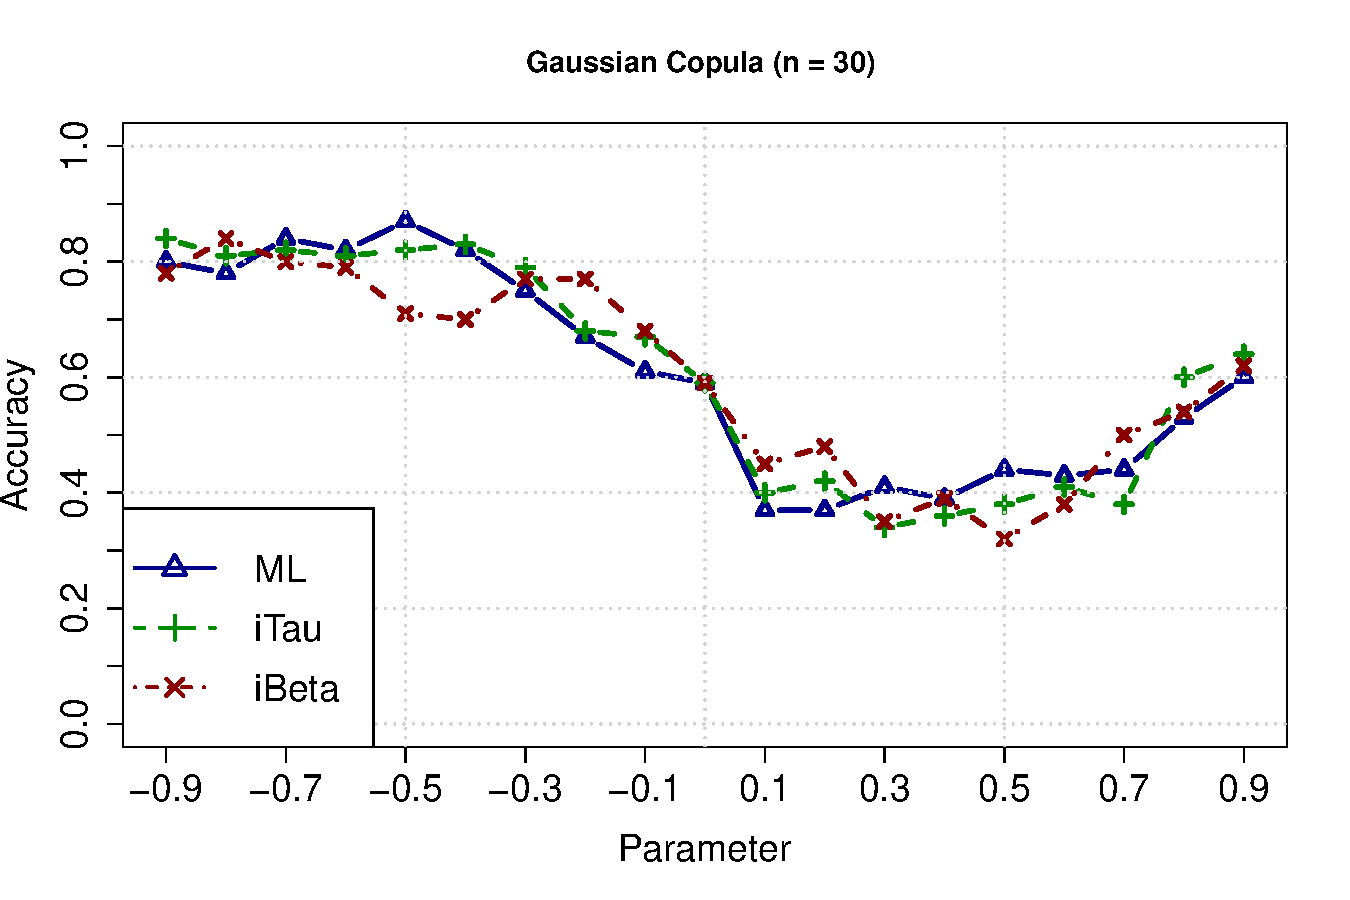
\includegraphics[trim= 0cm 0cm 1cm .7cm,clip=true, width = .48\textwidth]{Figures/mc-copSelection/gaussian-select30.pdf}
	}
	\hfill
	\subfloat{%
		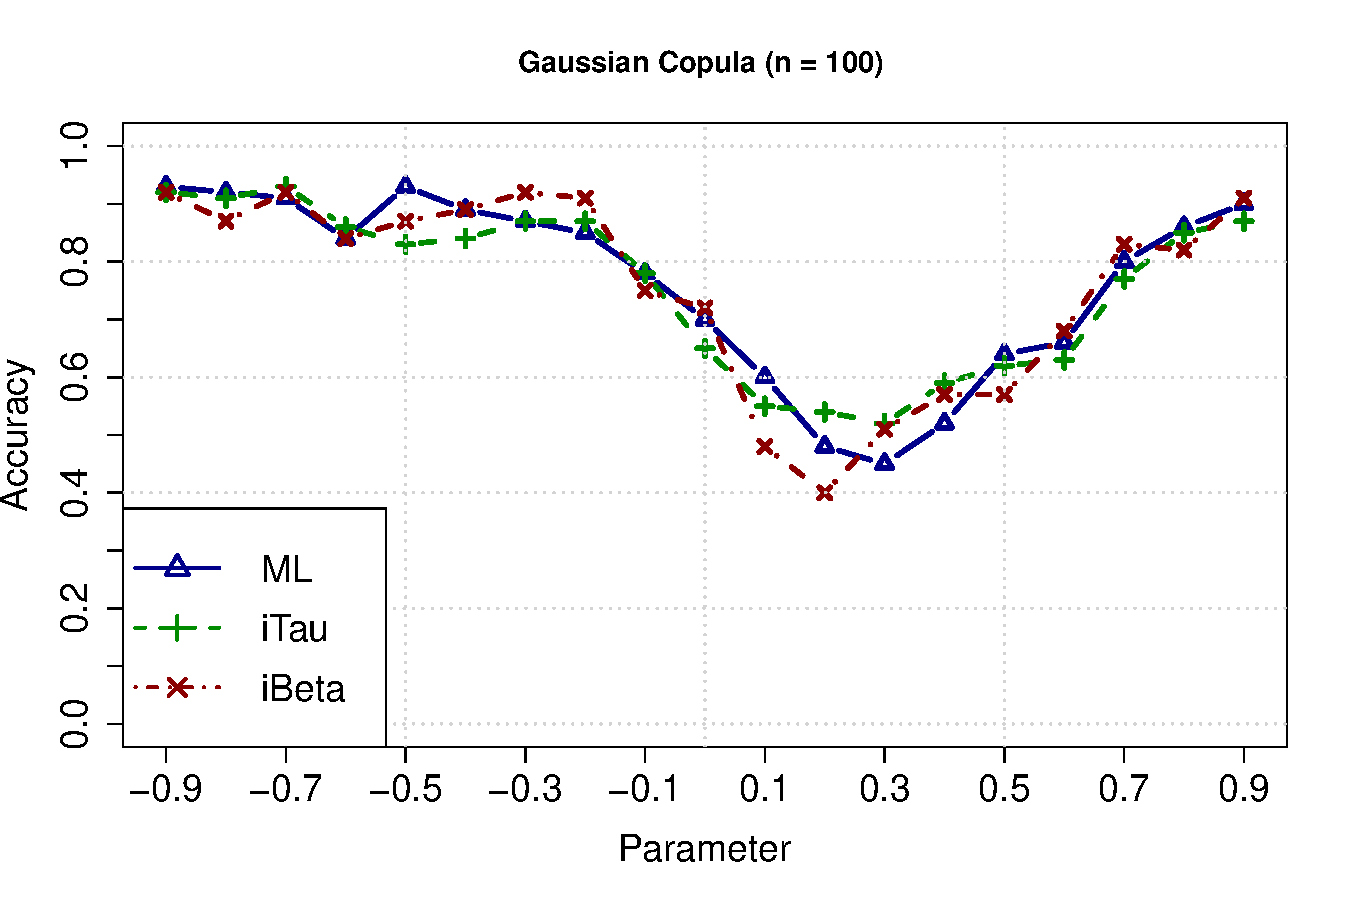
\includegraphics[trim= 0cm 0cm 1cm .7cm,clip=true,width = .48\textwidth]{Figures/mc-copSelection/gaussian-select100.pdf}
	}
	\hfill
	\subfloat{%
		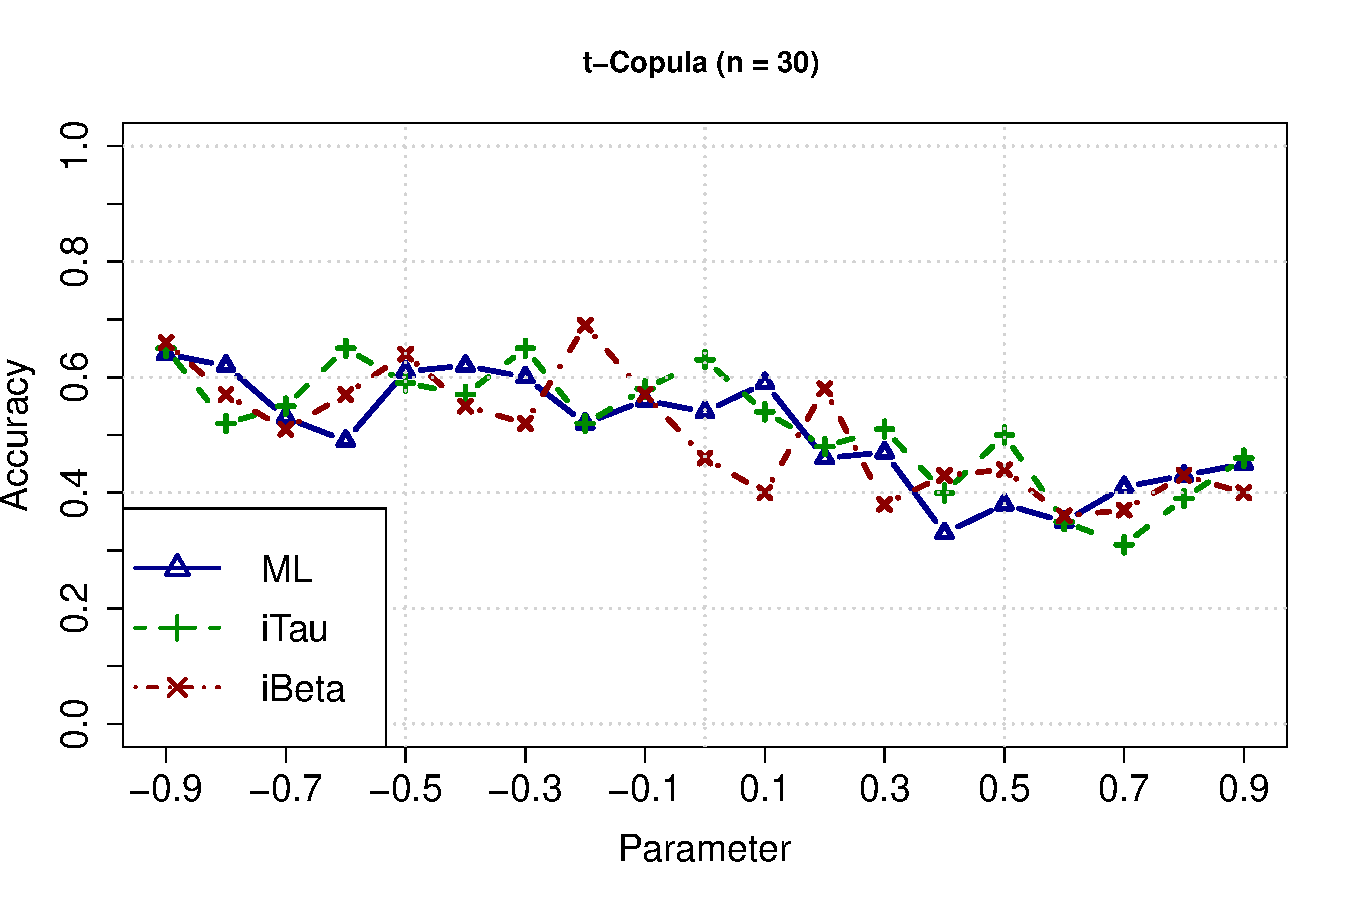
\includegraphics[trim= 0cm 0cm 1cm .7cm,clip=true,width = .48\textwidth]{Figures/mc-copSelection/t-select30.pdf}
	}
	\hfill
	\subfloat{%
		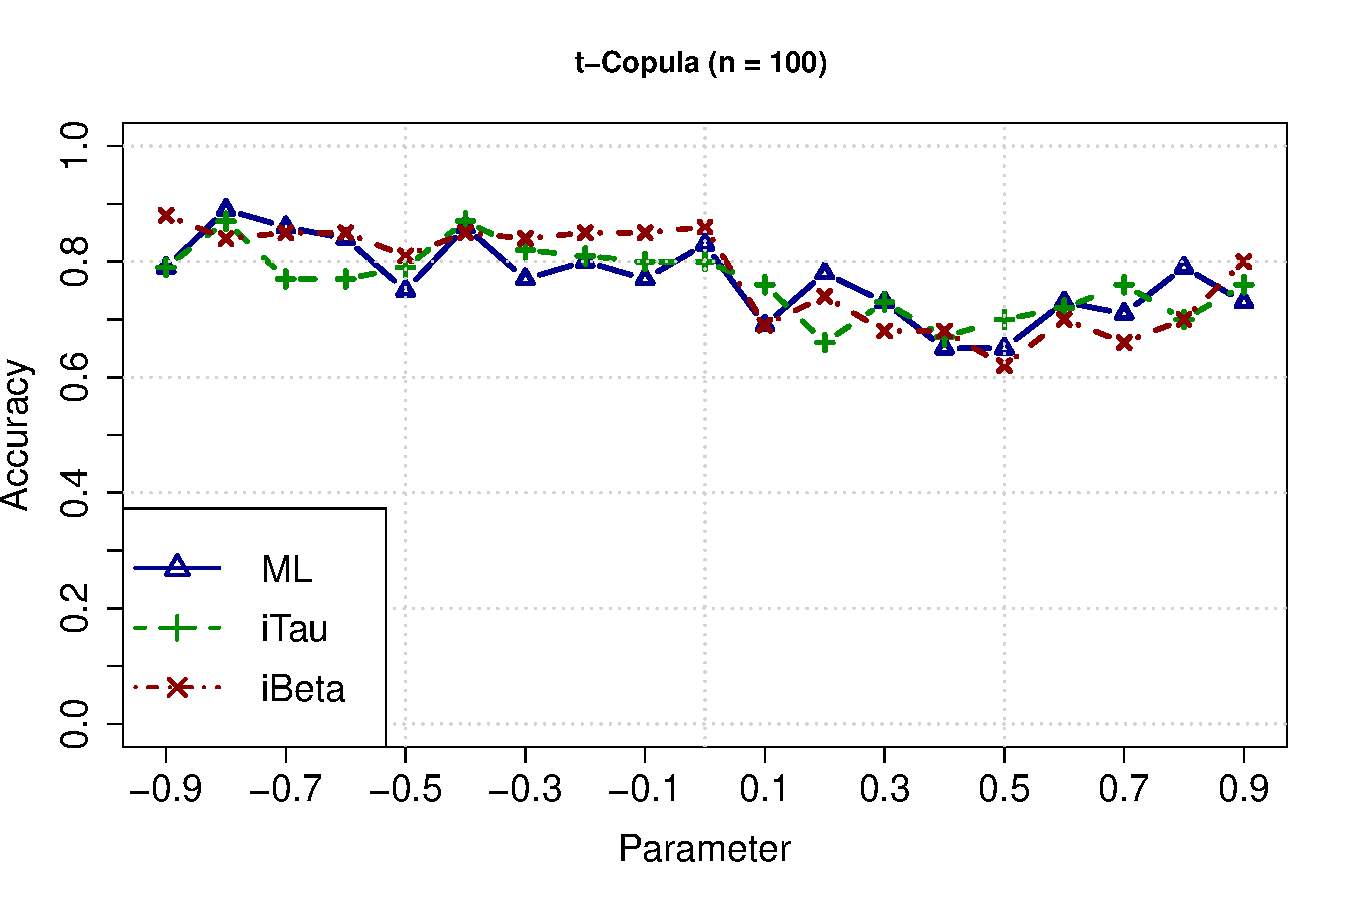
\includegraphics[trim= 0cm 0cm 1cm .7cm,clip=true,width = .48\textwidth]{Figures/mc-copSelection/t-select100.pdf}
	}
	\hfill
	\subfloat{%
		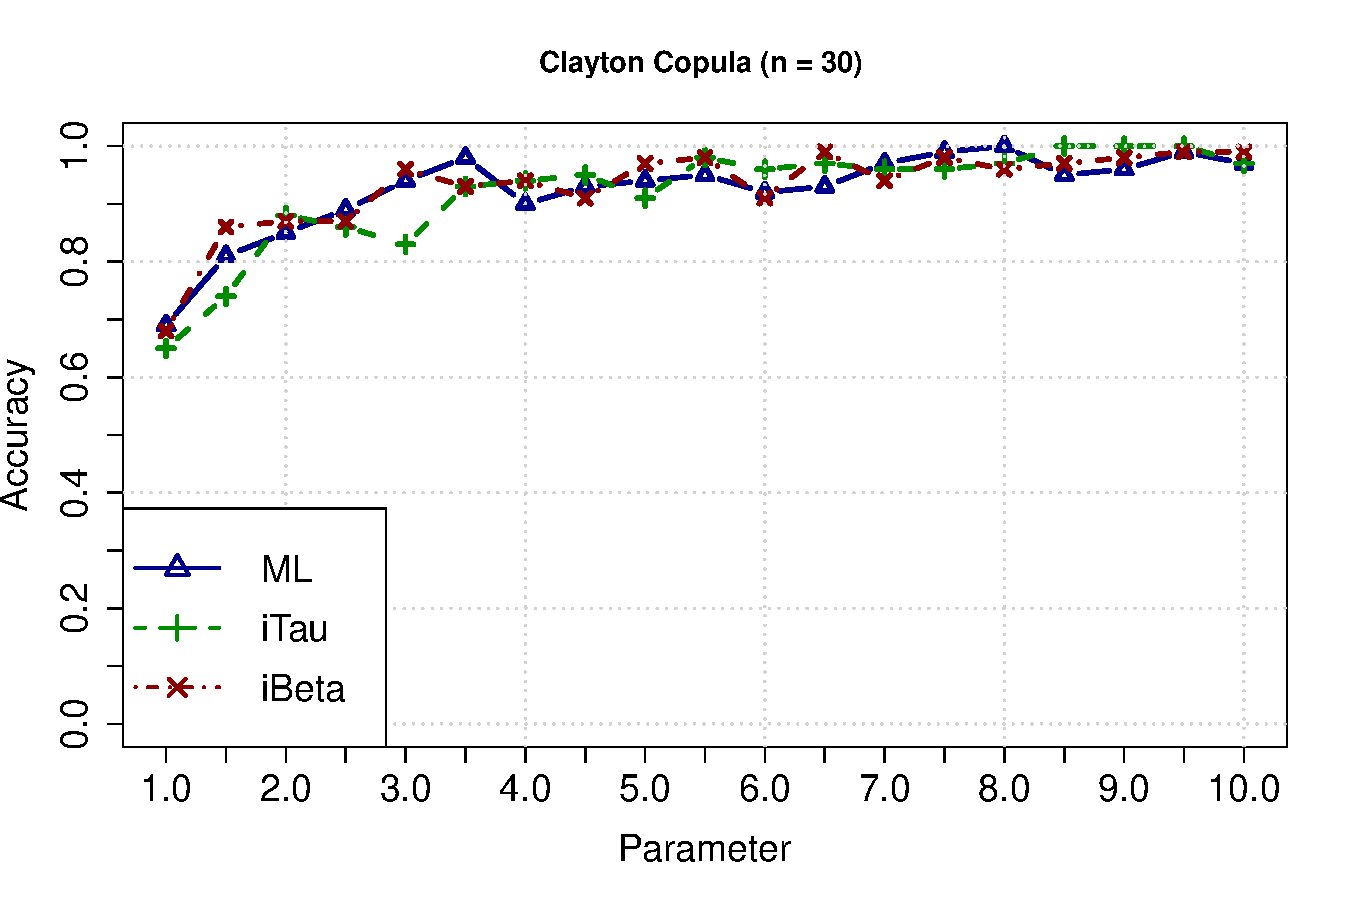
\includegraphics[trim= 0cm 0cm 1cm .7cm,clip=true,width = .48\textwidth]{Figures/mc-copSelection/clayton-select30.pdf}
	}
	\hfill
	\subfloat{%
		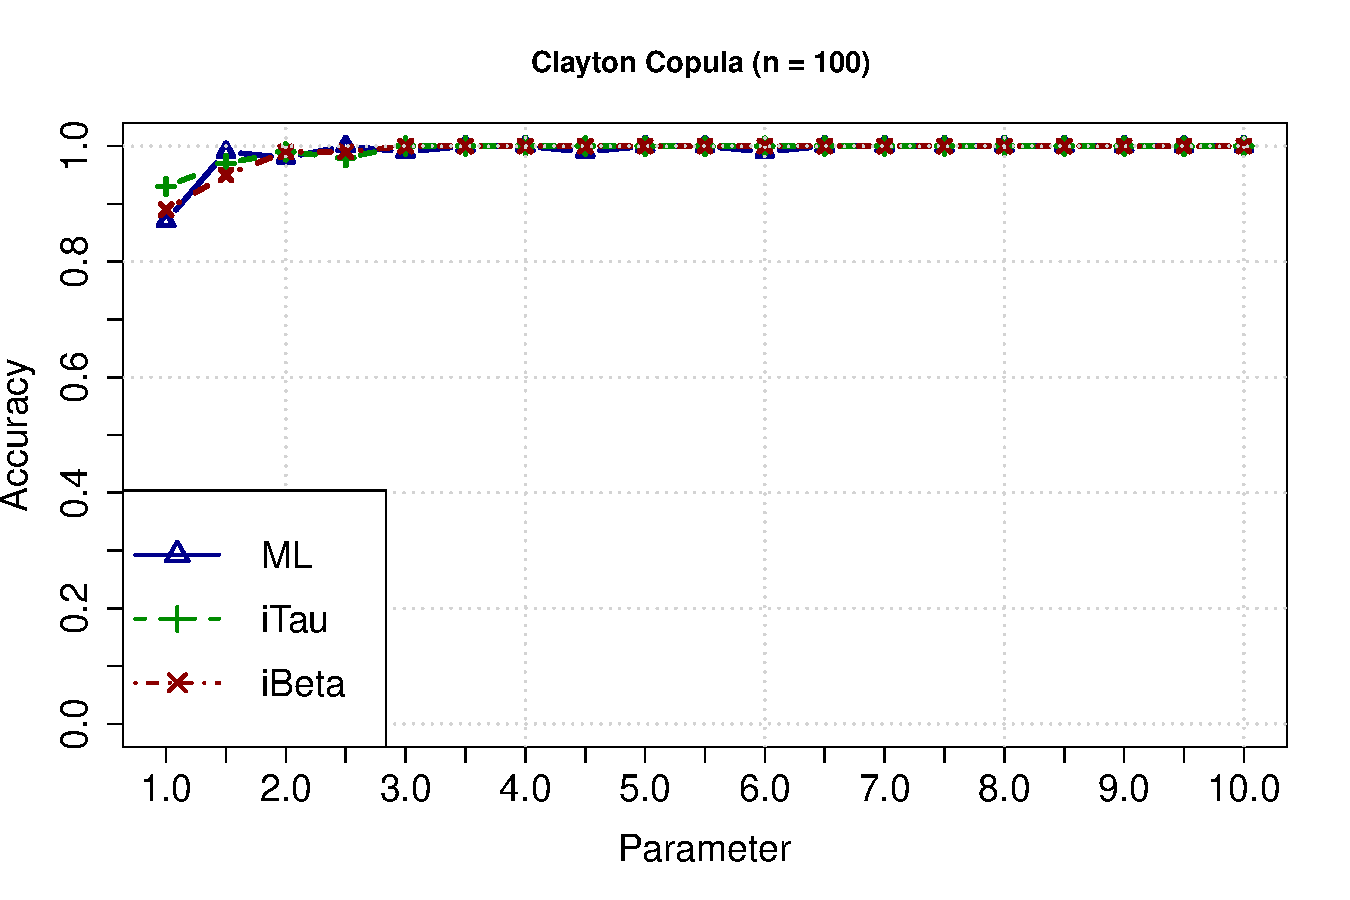
\includegraphics[trim= 0cm 0cm 1cm .7cm,clip=true,width = .48\textwidth]{Figures/mc-copSelection/clayton-select100.pdf}
	}
	\caption[\textsc{Accuracy of copula selection for different estimators / Gaussian, $t$ and Clayton copula}]{Accuracy of copula selection for different estimators with $ n = \left\lbrace 30,100 \right\rbrace $ and $k = 100$. Shown is the percentage of correct specifications per estimator, copula and parameter. This Figure images the behavior for the Gaussian, $t$, and Clayton copula.}
	\label{copSelect-gauss-t}
\end{figure}

\begin{figure}[t]
	\subfloat{%
		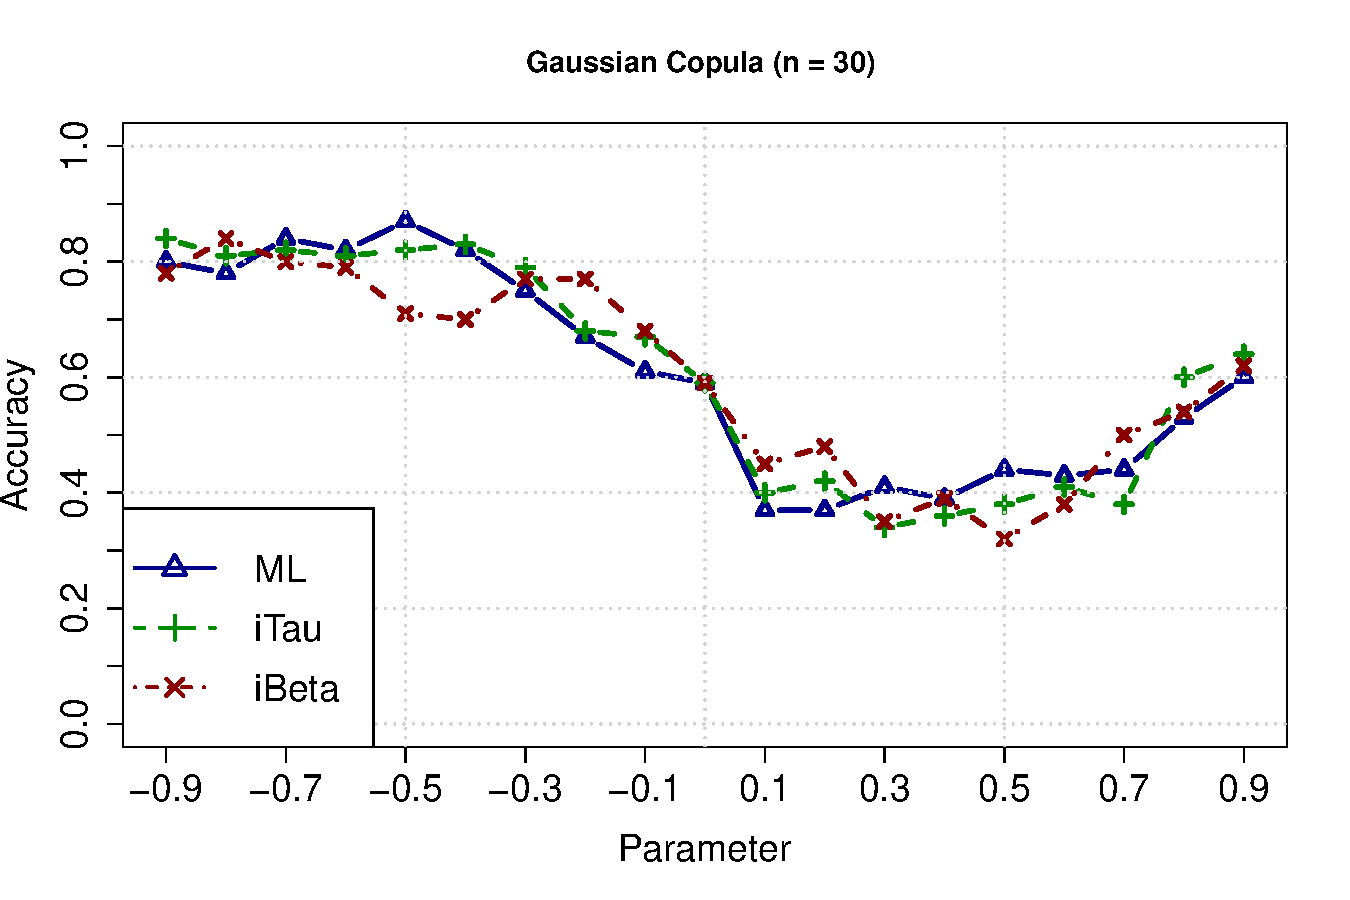
\includegraphics[trim= 0cm 0cm 1cm .7cm,clip=true, width = .48\textwidth]{Figures/mc-copSelection/gaussian-select30.pdf}
	}
	\hfill
	\subfloat{%
		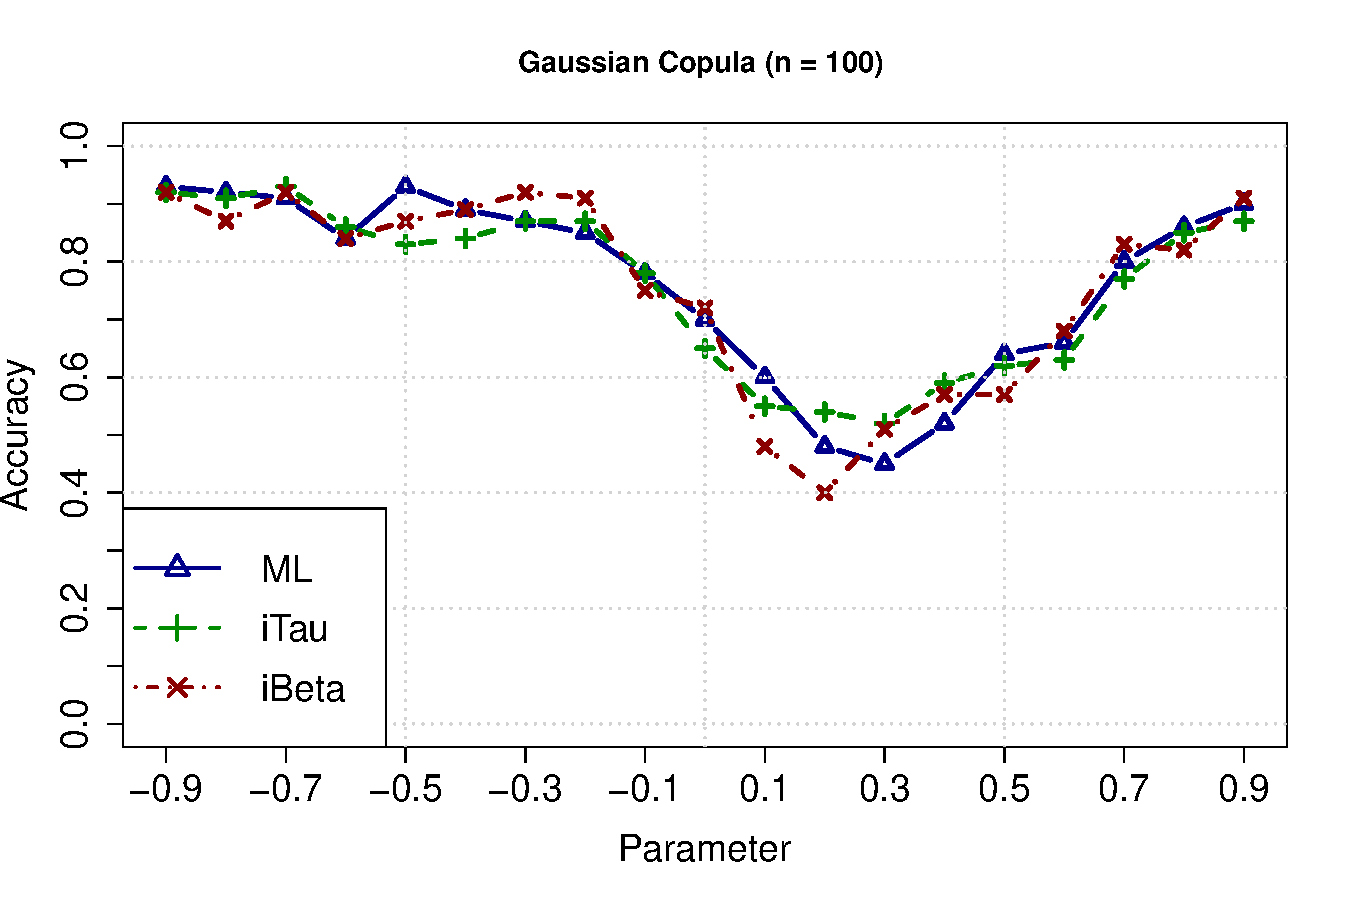
\includegraphics[trim= 0cm 0cm 1cm .7cmm,clip=true,width = .48\textwidth]{Figures/mc-copSelection/gaussian-select100.pdf}
	}
	\hfill
	\subfloat{%
		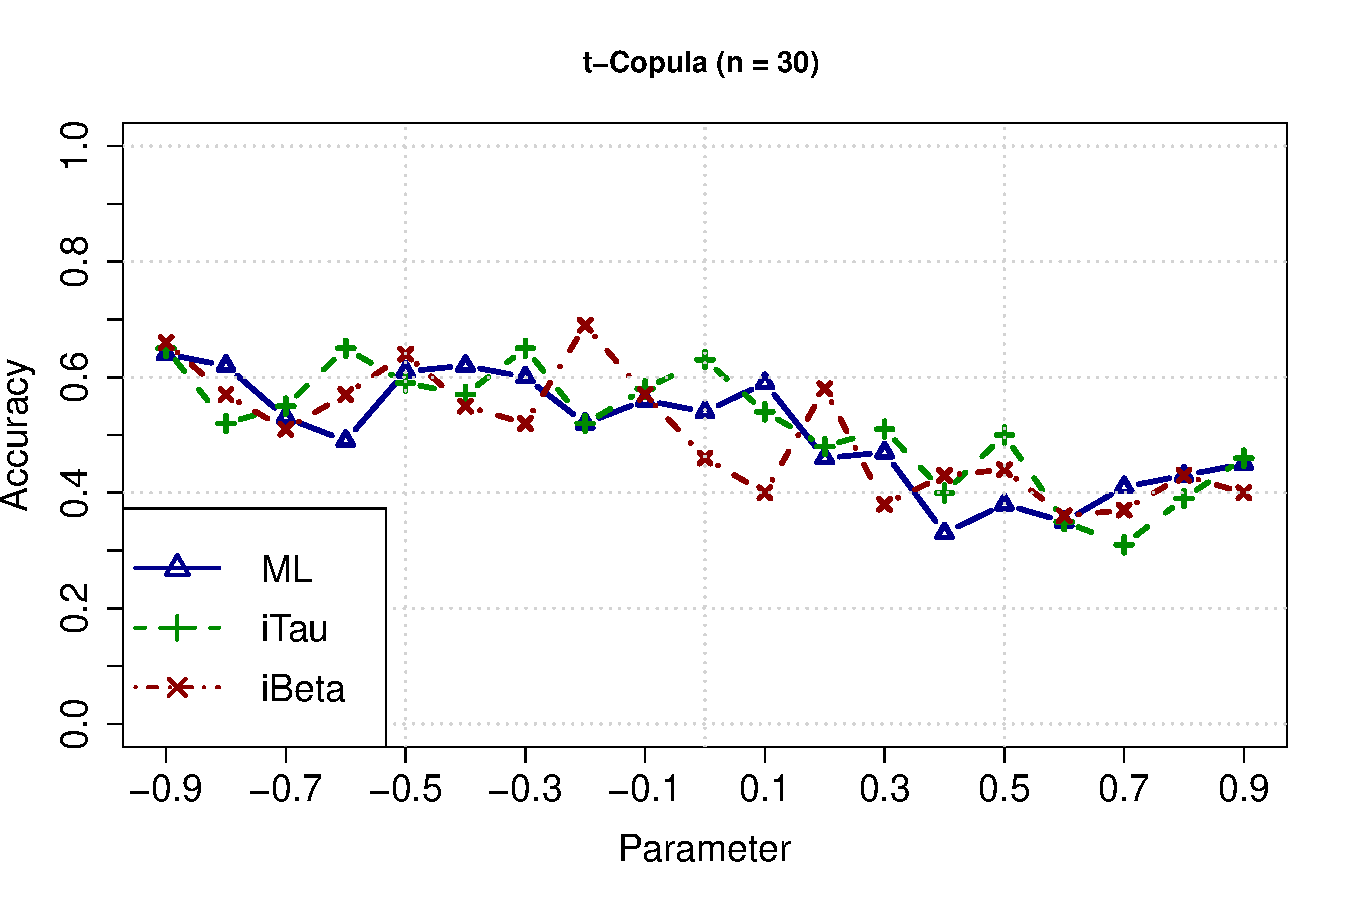
\includegraphics[trim= 0cm 0cm 1cm .7cm,clip=true,width = .48\textwidth]{Figures/mc-copSelection/t-select30.pdf}
	}
	\hfill
	\subfloat{%
		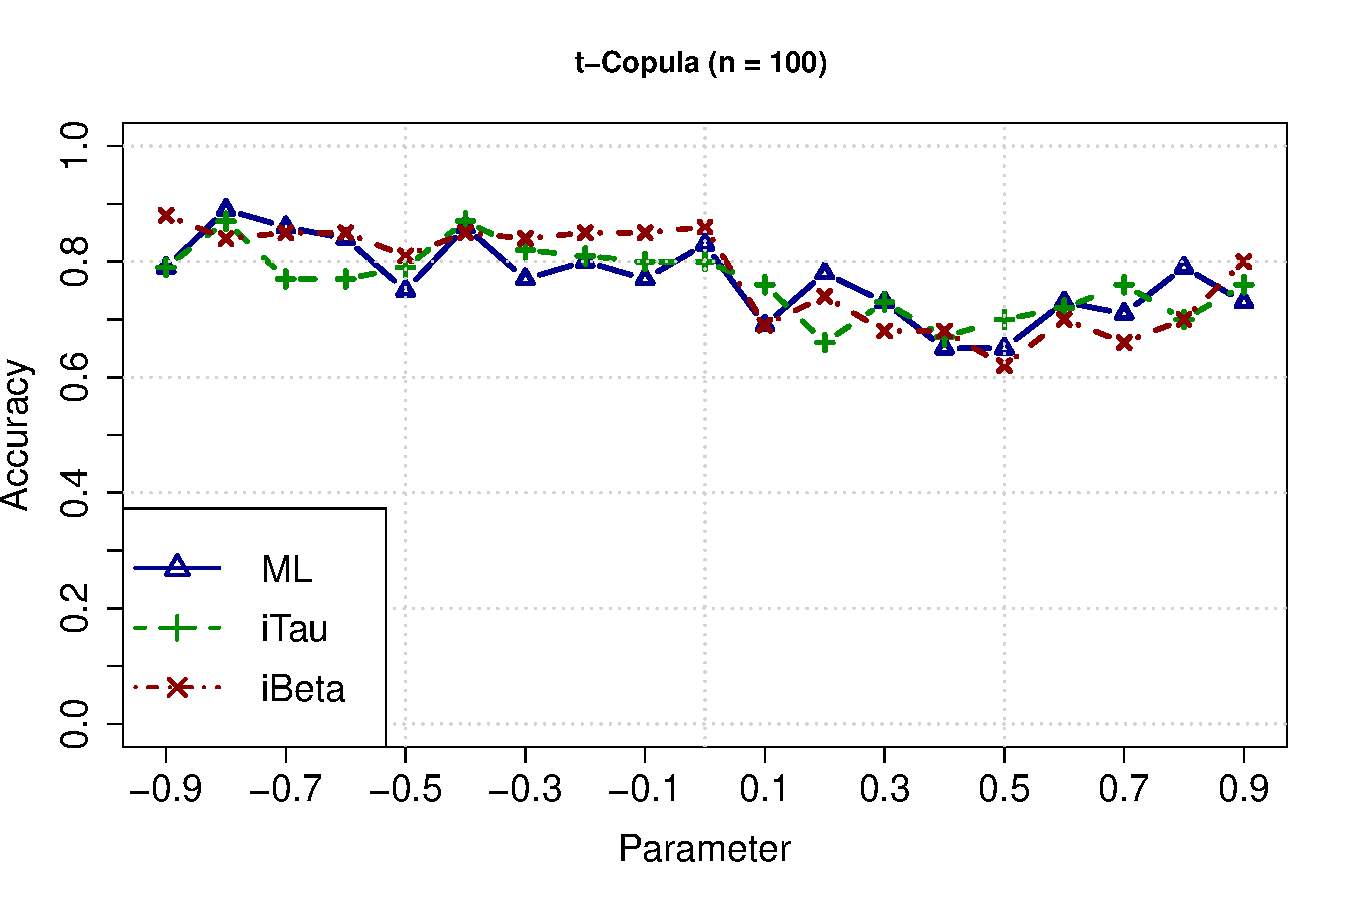
\includegraphics[trim= 0cm 0cm 1cm .7cm,clip=true,width = .48\textwidth]{Figures/mc-copSelection/t-select100.pdf}
	}
	\caption[\textsc{Accuracy of copula selection for different estimators / Gumbel and Frank copula}]{Continuation of Figure \ref{copSelect-gauss-t} for the Gumbel and Frank copula.}
	\label{copSelect-gumbel-frank}
\end{figure}


\begin{table}[h!]
	\centering
{\renewcommand{\arraystretch}{1.3}
	\begin{tabular}{ll|ccc}
		Copula family             & Estimator & $\min_t$   & $\tilde{t}$ & $\max_t$   \\ \hline \hline
		\multirow{3}{*}{Gaussian} & ML        & 0.666 & 1      & 3.706 \\
		& iTau      & 0.051 & 0.053  & 0.115 \\
		& iBeta     & 0.050 & 0.051  & 0.112 \\ \hline
		\multirow{3}{*}{t}        & ML        & 0.647 & 1      & 3.576 \\
		& iTau      & 0.050 & 0.051  & 0.159 \\
		& iBeta     & 0.048 & 0.049  & .0125 \\ \hline
		\multirow{3}{*}{Clayton}  & ML        & 0.606 & 1      & 2.936 \\
		& iTau      & 0.040 & 0.041  & 0.090 \\
		& iBeta     & 0.039 & 0.040  & 0.084 \\ \hline
		\multirow{3}{*}{Gumbel}   & ML        & 0.643 & 1      & 2.638 \\
		& iTau      & 0.059 & 0.061  & 0.086 \\
		& iBeta     & 0.058 & 0.059  & 0.104 \\ \hline
		\multirow{3}{*}{Frank}    & ML        & 0.670 & 1      & 3.288 \\
		& iTau      & 0.044 & 0.045  & 0.100 \\
		& iBeta     & 0.042 & 0.043  & 0.076
	\end{tabular}
}
\caption[Relative computation time per copula and estimator for copula selection]{Relative computation time per copula and estimator for the selection process. Time is measured relative to the median time it takes the maximum likelihood estimator in combination with the AIC to find an optimal copula. $n$ has been set to $100$ and $k = 1000$. }
\label{comp-time-seletion}
\end{table}

\section{Conclusion}

This study compared the performance and accuracy of three different estimators regarding parameter estimation and selection of copulae. Concerning the first one, the results of previous studies could be reproduced, finding that for accurate estimation of a copula's parameter the maximum likelihood estimator remains the mean of choice. Both moment based estimators, especially Blomqvist's Beta are significantly worse in estimating, however, are considerably faster computationally. Hence, one could use those estimators to perform a quick-and-dirty estimation to find a starting value for a subsequent ML estimation. This poses the interesting question of how much more efficient such a procedure would be in comparison to only use ML.

In a second step a fast procedure for selecting copulae could be found. The accuracy when selecting copulae remains almost equal across all copulae, parameters and sample sizes for every estimator. In terms of algorithmic complexity, the moment-based estimators stand out, as they only need a fraction of the time ML needs to select a copula from arbitrarily generated data. Therefore, it seems reasonable to prefer those over ML, especially in large sample size or big-data environments. The \verb*|R| workspace and functions can be provided upon request.

With over $855,000$ parameter estimations and around $57,000$ copula selections computed in this study, it counts to the more comprehensive ones carried out so far, yet there are also drawbacks. I only implemented the selection process for five copulae and three estimators, so it would be an interesting task to realize the selection algorithm for the remaining copulae and also test its performance. A real-world application putting the algorithm to use is also pending. 